\section{Datenbankdesign}

Dieses Projekt wurde mit eines MySQL Datenbank auf Version 5.7.23 realisiert. Es wurden zuerst die geforderten Entitäten aus der Angabe extrahiert und mithilfe eines grafischen Modellierungswerkzeugs namens MySQL Workbench 8\footnote{https://dev.mysql.com/downloads/workbench/} modelliert.

\begin{figure}[H]
\centering
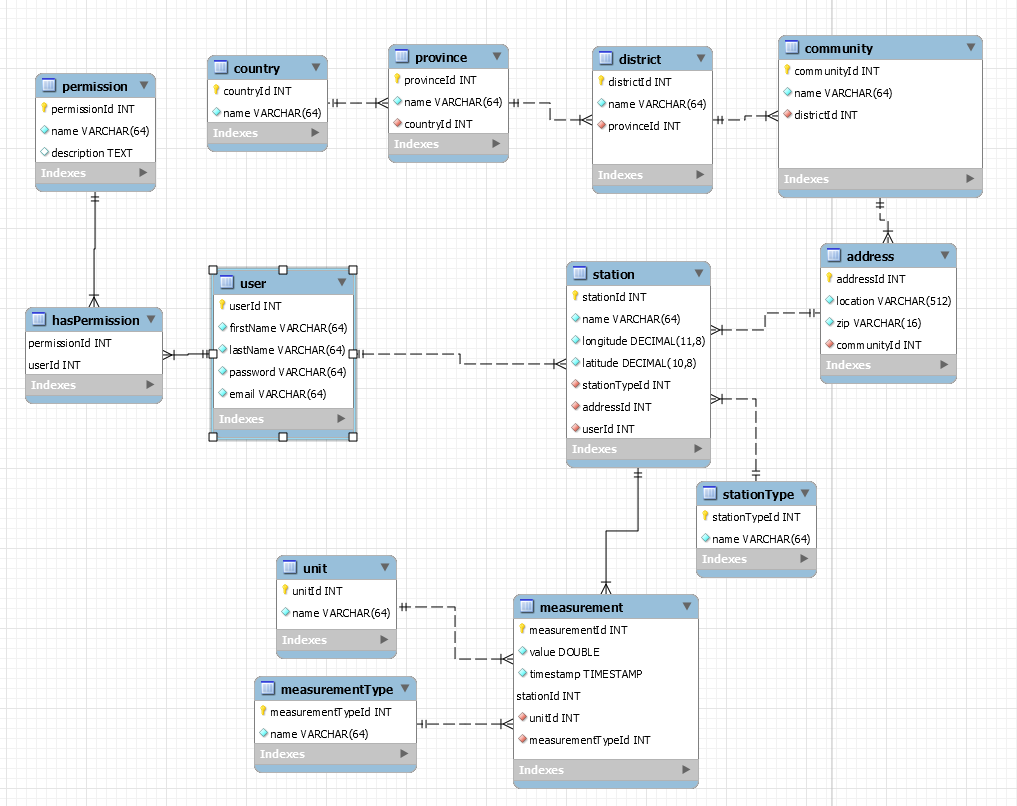
\includegraphics[width=.85\textwidth]{database.png}
\caption{Datenbankschema des Wetr-Projekts in der ersten Ausbaustufe.}
\label{fig:db}
\end{figure}
\raggedright
Wie in Abbildung \ref{fig:db} zu sehen wird zur Verwaltung des Standortes einer Station eine Reihe von abhängigen Entitäten verwendet. Um die Flexibilität zu erhöhen wurde neben zusätzlich ein \textit{Country} modelliert. In einem \textit{Country} befinden sich \textit{Provinces}, welche Bundesländer darstellen. Jede \textit{Province} wird in mehrere \textit{Districts} unterteilt, ähnlich wie Bezirke. In jedem \textit{District} gibt es mehrere \textit{Communities}, welche mit Gemeinden vergleichbar sind. Als kleinste Entität in dieser Kette gibt es die \textit{Address}, welche einen einfachen String zur Angabe von genaueren Addressdaten (rein zur Anzeige oder falls anderswo benötigt) und eine Zuordnung mittels Postleitzahl enthält.\\
Im Datenbankschema gibt es \textit{User}, welche, falls benötigt, verschiedene \textit{Permissions} zugewiesen haben können. Ein \textit{User} kann mehrere \textit{Stations} betreiben, welche wiederum neben der \textit{Address} auch einen Namen und die Geokoordinaten in Form von Latitide und Longitude gespeichert hat. Der Typ der Station wurde in eine eigene Entität \textit{StationType} ausgelagert.\\
Jede \textit{Station} kann beliebig viele \textit{Measurements} generieren, welche neben den ebenfalls ausgelagerten Entitäten \textit{MeasurementType} und \textit{Unit}, auch einen Zeitstempel und dazugehörigen Messwert besitzen.\\

\subsection{Beispieldaten Generierung}

\subsubsection{Stationen, Addressen und Communities}

Der \textit{Extractor} (befindet sich im extractor Ordner) wurde mit Python\footnote{https://www.python.org/} geschrieben und verwendet die Stationsliste der \textit{Zentralanstalt für Meteorologie und Geodynamik}\footnote{https://www.zamg.ac.at/cms/de/klima/messnetze/wetterstationen}. Die \grqq{}.csv\grqq{} Datei wird vom Extractor eingelesen und für jede \textit{Station} wird eine Insert Anweisung in eine \grqq{}.txt\grqq{} Datei geschrieben. Zusätzlich wird anhand des Längen- und Breitengrades der Ort mit einem geolocator der Aufenthaltsort der Station ermittelt. Anhand dieser Daten werden SQL Anweisungen für die \textit{Community} und \textit{Address} Tabellen erstellt die von der jeweiligen Stationen referenziert werden.

\subsubsection{Messdaten}
Für die erste Ausbaustufe dieses Projekts wurde ein Generator implementiert, der über eine Millionen Messdaten generiert. Diese Messdaten sind jedoch nicht realitätsnahe, sondern haben als Basis den Jahresdurchschnitt in Österreich laut Klimatabelle\footnote{https://www.klimatabelle.info/europa/oesterreich}.
Für eine genauere Beschreibung siehe Abschnitt \ref{sec:generator}.

\subsubsection{Andere Daten}
Die Beispieldaten der restlichen Tabellen wurden per Hand mithilfe vom Internet zusammengestellt. \textit{Provinces}, \textit{Districts} und weiter Standortbezogene Daten sind höchstwarhscheinlich nicht vollständig übernommen worden.